\scanpage{4}
\mspage{3}
façon particulièrement jolie de les raccorder, de façon à reconstituer \deleted{une}\inserted{l'}affinisation supercritique de $\underline\Sigma$ sur $F_i$. On trouve une surface $\mathcal X'_1$, où les sommets \deleted{\unsure{supercri}}\inserted{sur les} faces supersingulières sont d'ordre $3$, tous les autres sommets étant d'ordre $4$. Il faudrait expliciter les arcs de spécialisation (et \unsure{aussi|non}, symétriquement, de générisation sur les $\widetilde D_i$), non seulement sur les p.r. sous-stables voisines de $D_i$, mais maintenant aussi sur les p.r. stables voisines. Cette fois, on a des arcs de spécialisation de longueur combinatoire $\frac12$ --- ce qui amène à introduire la subdivision barycentrique \unsure{itérée double} de la subdivision cellulaire qu'on a sur les $\widetilde D$ et les $\widetilde D_i$. \deleted{Et}

\figure{%
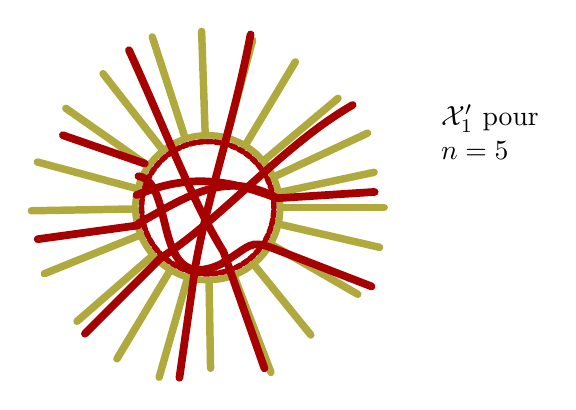
\begin{tikzpicture}[scale=.8,line cap=round]
\draw[yellow!65!black,line width=2.4pt](0,0)circle(1.15);
\foreach \a/\r in {0/2.8,12/2.7,25/2.8,40/2.7,59/2.7,75/2.75,92/2.8,108/2.85,128/2.7,145/2.75,165/2.8,181/2.8,202/2.8,221/2.75,239/2.8,254/2.8,271/2.55,291/2.8,309/2.6,330/2.75,347/2.8}{\draw[yellow!65!black,line width=2.7pt](\a:1.15)--(\a:\r);}
\draw[red!65!black,densely dotted,line width=2pt](0,0)circle(1.05);
\draw[red!65!black,line width=2.8pt] (-1.13,.2)..controls(-.4,.5)and(.2,.5)..(1.1,.15)--(2.65,.25) (-1.1,-.28)--(-2.7,-.5);
\draw[red!65!black,line width=2.8pt] (-1.1,-.25)..controls(-.3,.2)and(.3,.6)..(1.1,.15);
\draw[red!65!black,line width=2.8pt] (-1.25,2.5)..controls(-.7,1.3)and(-.25,.1)..(.25,-.7)--(.9,-2.55);
\draw[red!65!black,line width=2.8pt] (.68,2.75)..controls(.4,1.3)and(.0,.2)..(-.2,-.95)--(-.45,-2.7);
\draw[red!65!black,line width=2.8pt] (2.3,1.63)..controls(1.2,1)and(.2,-.2)..(-.75,-.8)--(-1.95,-2.0);
\draw[red!65!black,line width=2.8pt] (-1.1,.5)..controls(-.5,.4)and(-.9,-1.4)..(.2,-.9)..controls(.7,-.6)and(.65,-.5)..(1.05,-.65)--(2.6,-1.25);
\draw[red!65!black,line width=2.8pt](-2.3,1.15)--(-1.0,.7);
\node[right,align=left]at(3.55,1.2){$\mathcal X'_1$ pour\\$n=5$};
\end{tikzpicture}%
}

Le défaut commun \deleted{aux}\inserted{à ces} trois surfaces représentatives $\mathcal X_0$, $\mathcal X_1$, $\mathcal X'_1$ pour les p.rel. est que le système local, ou transport parallèle, des \deleted{$\unsure{D}$} \unsure{polygônes|polygones} combinatoires $\operatorname{Pol}(D)$ n'est défini ici que sur le complémentaire de l'union des \deleted{\unsure{faces}}\inserted{sommets}, ou faces supercritiques, qui sont des lieux de ramification effective.
Un autre défaut, sans doute apparenté, est qu'on n'a pas d'\unsure{application|injection} naturelle de ces surfaces dans $X$, sauf erreur (\deleted{sauf erreur} peut-être dans le cas de $\mathcal X'_1$ --- à regarder de façon \deleted{plus} détaillée\ldots). C'est pour pallier à ce (ou ces) défauts qu'il peut être
\margin{3}
